\documentclass[10pt,a4paper]{article}
\usepackage[a4paper,margin=2cm,top=2.2cm,bottom=2.2cm]{geometry}
\usepackage[T1]{fontenc}
\usepackage[utf8]{inputenc}
\usepackage[scaled=0.92]{helvet}
\renewcommand{\familydefault}{\sfdefault}
\usepackage{microtype}
\usepackage{graphicx}
\usepackage{booktabs}
\usepackage{xcolor}
\usepackage[font=small,labelfont=bf,skip=4pt]{caption}
\usepackage{titlesec}
\usepackage{enumitem}
\usepackage[most]{tcolorbox}
\usepackage{fancyhdr}
\usepackage[hidelinks]{hyperref}

\definecolor{accent}{HTML}{0072B2}
\definecolor{soft}{HTML}{F1F0EA}
\definecolor{muted}{HTML}{5A5A5A}
\graphicspath{{figures/}}
\setlength{\parindent}{0pt}
\setlength{\parskip}{5pt}
\titleformat{\section}{\large\bfseries\color{accent}}{\thesection}{0.6em}{}
\titlespacing*{\section}{0pt}{10pt}{3pt}
\setlist[itemize]{leftmargin=1.2em,itemsep=2pt,topsep=2pt,parsep=0pt}
\pagestyle{fancy}\fancyhf{}
\renewcommand{\headrulewidth}{0pt}
\fancyfoot[L]{\footnotesize\color{muted}SENSE energy: day-ahead demand forecasting for NHS sites}
\fancyfoot[R]{\footnotesize\color{muted}\thepage}
\newcommand{\tablefont}{\small\renewcommand{\arraystretch}{1.08}}
\newsavebox{\figa}\newsavebox{\figb}
% two figures in one row at a common height; #1 = share of the text width (default 0.98)
\newcommand{\pair}[3][0.98]{%
  \sbox{\figa}{\includegraphics[height=5cm]{#2}}%
  \sbox{\figb}{\includegraphics[height=5cm]{#3}}%
  \begin{center}\resizebox{#1\textwidth}{!}{\usebox{\figa}\hspace{0.5cm}\usebox{\figb}}\end{center}}
% a figure block that never separates from its caption
\newenvironment{figblock}{\par\medskip\noindent\begin{minipage}{\textwidth}}{\end{minipage}\par\medskip}

\raggedbottom
\begin{document}

{\LARGE\bfseries\color{accent} Day-ahead energy demand forecasting\\[2pt] for NHS sites}\\[4pt]
{\large Results to date}\hfill{\color{muted}SENSE energy \textbullet\ 29 September 2026}
\vspace{2pt}\hrule\vspace{6pt}

\begin{tcolorbox}[colback=soft,colframe=soft,boxrule=0pt,arc=2pt,left=6pt,right=6pt,top=5pt,bottom=5pt]
\textbf{Key results}
\begin{itemize}
\item Half-hourly electricity demand of an NHS site can be forecast a day ahead with a normalised error of \textbf{11.5\,\%}, against 18.5\,\% for seasonal naive. The gain holds on 99\,\% of sites.
\item \textbf{Foundation models used without any training on NHS data lead}: Chronos-2 and TimesFM~3.0 beat a trained LightGBM model and SARIMA.
\item Known-ahead covariates (calendar, price, grid forecasts, weather) improve every model family by about 0.7 points. \textbf{Forecast weather is as good as perfect weather} at this range.
\item The 51-member weather ensemble does not change the demand distribution, but its spread identifies the days with the largest errors.
\item Reconciling forecasts across the hierarchy gives coherent numbers from meter to national level and lowers the national error from 8.0\,\% to \textbf{6.8\,\%}.
\item Sites fall into three demand shapes set by their function, not by the type of trust. Electricity demand changes by only 1 to 2\,\% per degree.
\end{itemize}
\end{tcolorbox}

\section{Experiment}
The target is the half-hourly electricity demand of 91 NHS sites in England, those with at least 85\,\% of readings observed and a year of history, drawn from 134 sites and 24 trusts. Each forecast is issued at 16:30 local time and covers the 48 half-hours of the following day. The test window runs from June 2025 to May 2026 with 69 forecast days that rotate through the weekdays, giving 6,279 site-days.

Scores use observed readings only. nMAE is the mean absolute error divided by the site's mean demand. CRPS, in kWh per half hour, scores the whole predictive distribution on nine quantiles. Coverage is the share of observations inside the nominal 80\,\% interval. Skill is the relative improvement over seasonal naive, the value one week earlier.

\section{Accuracy at site level}
\begin{figblock}\centering\tablefont
\begin{tabular}{lrrrrr}
\toprule
Method & nMAE (\%) & CRPS & Coverage (\%) & CRPS skill (\%) & Sites better than naive (\%) \\
\midrule
Seasonal naive & 18.5 & 12.93 & -- & -- & -- \\
Profile quantiles & 18.3 & 9.99 & 60 & 23 & 64 \\
SARIMA & 18.9 & 9.24 & 82 & 17 & 53 \\
\addlinespace[3pt]
LightGBM & 13.4 & 6.41 & 74 & 41 & 97 \\
LightGBM + ERA5 & 12.8 & 6.16 & 73 & 44 & 97 \\
LightGBM + IFS ENS & 13.1 & 6.27 & 73 & 43 & 97 \\
\addlinespace[3pt]
Chronos-2 & 12.2 & 5.37 & 76 & 45 & 99 \\
Chronos-2 + ERA5 & \textbf{11.5} & 5.14 & 76 & 48 & 99 \\
Chronos-2 + IFS ENS & \textbf{11.5} & \textbf{5.13} & 75 & 48 & 99 \\
\addlinespace[3pt]
TimesFM 3.0 & 12.4 & 5.46 & 81 & 44 & 99 \\
TimesFM 3.0 + ERA5 & 11.6 & 5.32 & 81 & 48 & 99 \\
TimesFM 3.0 + IFS ENS & 11.7 & 5.35 & 81 & 48 & 99 \\
\addlinespace[3pt]
TabPFN-TS & 14.1 & 6.68 & 76 & 38 & 98 \\
TabPFN-TS + ERA5 & 12.0 & 5.71 & 77 & 47 & 99 \\
TabPFN-TS + IFS ENS & 12.1 & 5.74 & 77 & 46 & 99 \\
\bottomrule
\end{tabular}

\captionof{table}{Day-ahead results pooled over 91 sites and 69 forecast days. ``+ ERA5'' adds the known-ahead covariates with reanalysis weather, which is perfect weather; ``+ IFS ENS'' uses the weather forecast available at issue time. CRPS skill is the median across sites. Best values in bold.}
\end{figblock}

LightGBM and the three foundation models improve on seasonal naive by 38 to 48\,\% in CRPS. Chronos-2 and TimesFM~3.0 lead with demand history alone, and the covariates lift all four model families. TabPFN-TS gains most, because its own features carry no weather. SARIMA, refitted at every forecast day, is no more accurate than naive on the median site: it does well on large regular sites and fails on small erratic ones.

\begin{figblock}
\pair{crps_skill_by_method}{covariate_gain}
\captionof{figure}{Left: CRPS skill against seasonal naive for each method. Right: change in CRPS skill from adding covariates, paired per site against the same model without them. Markers show the median across sites and lines the interquartile range. Circles are models without covariates, squares use reanalysis weather and triangles forecast weather; the inverted triangle and the diamond are Chronos-2 with the control member and with all 51 members.}
\end{figblock}

\section{Probabilistic quality and the weather ensemble}
TimesFM~3.0 is calibrated, with 81\,\% of observations inside its 80\,\% interval. Chronos-2 and TabPFN-TS are slightly narrow at 75 to 77\,\%, and LightGBM is narrow at 73\,\%.

\begin{figblock}\centering\tablefont
\begin{tabular}{lrrr}
\toprule
Weather given to Chronos-2 & nMAE (\%) & CRPS & Coverage (\%) \\
\midrule
No covariates & 12.20 & 5.372 & 76 \\
\addlinespace[3pt]
Ensemble mean & 11.54 & 5.132 & 75 \\
Control member & 11.55 & 5.136 & 76 \\
51 members, mixed & 11.54 & 5.135 & 75 \\
\addlinespace[3pt]
Reanalysis (perfect weather) & 11.49 & 5.139 & 76 \\
\bottomrule
\end{tabular}

\captionof{table}{Chronos-2 with the same covariates and different weather inputs.}
\end{figblock}

Running Chronos-2 once per ensemble member and mixing the 51 resulting distributions gives the same scores as using the ensemble mean or the control member. Member forecasts differ by 0.6\,\% of mean demand on the median site-day, far less than the width of the model's own interval. The spread is nonetheless informative: the error of the forecast rises from 3\,\% to 30\,\% of mean demand between the lowest and highest tenth of spread.

\begin{figblock}
\pair[0.86]{calibration}{ensemble_spread_skill}
\captionof{figure}{Left: observed frequency below each predicted quantile, pooled over sites and periods; the dashed diagonal is perfect calibration. Right: error of the member-mean forecast against the spread of the 51 member medians, in tenths of the spread distribution.}
\end{figblock}

\section{When and where errors occur}
Errors are largest on the working-day plateau, between 09:00 and 16:00, and smallest at night. Skill is positive almost everywhere on the map and is highest at the large acute sites. Regional totals range from 2.8\,\% nMAE in the East of England to 15.5\,\% in the South West. The two weakest regions are each dominated by one large site with days on which recorded demand halves.

\begin{figblock}
\pair[0.9]{nmae_by_hour}{map_site_skill}
\captionof{figure}{Left: normalised error by local time of the target day for the models without covariates and the baselines. Right: CRPS skill of Chronos-2 with forecast weather at each site, with marker area proportional to mean demand.}
\end{figblock}

\begin{figblock}
\begin{center}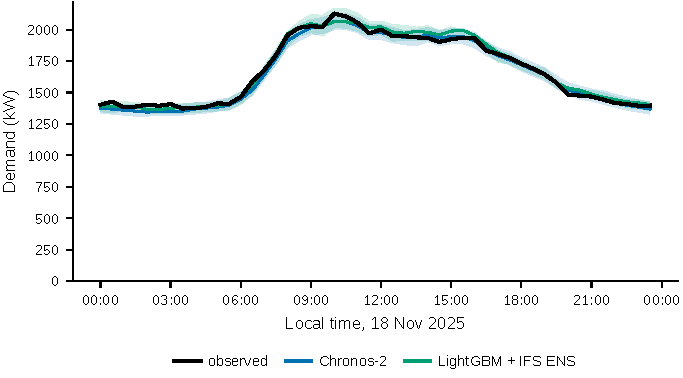
\includegraphics[width=0.66\textwidth]{example_day}\end{center}
\captionof{figure}{The largest site on one target day: observed demand with the predictive medians and 80\,\% intervals of Chronos-2 and of LightGBM with forecast weather.}
\end{figblock}

\section{Hierarchy and reconciliation}
The data form an exact hierarchy: meters sum to sites, sites to trusts, trusts to NHS regions and regions to the national total of the 91 sites. Forecasting each level directly becomes more accurate with aggregation.

\begin{figblock}\centering\tablefont
\begin{tabular}{lrrrrr}
\toprule
Direct forecast & Meter & Site & Trust & Region & National \\
\midrule
\textit{Series} & \textit{111} & \textit{91} & \textit{19} & \textit{6} & \textit{1} \\
\addlinespace[3pt]
Seasonal naive & 18.7 & 18.5 & 16.3 & 16.7 & 15.0 \\
LightGBM + IFS ENS & 13.0 & 13.1 & 10.3 & 10.0 & 9.0 \\
TimesFM 3.0 + IFS ENS & 11.7 & 11.7 & 8.7 & 8.6 & 8.0 \\
Chronos-2 + IFS ENS & 11.6 & 11.5 & 8.4 & 8.5 & 8.0 \\
\bottomrule
\end{tabular}

\captionof{table}{nMAE (\%) of direct forecasts at each level.}
\end{figblock}

Direct forecasts at different levels do not add up. Reconciliation maps them to a coherent set. Eight approaches were compared on the same 61 forecast days, with the variance-based approaches learning only from errors on earlier days.

\begin{figblock}\centering\tablefont
\begin{tabular}{lrrrrr}
\toprule
Approach & Meter & Site & Trust & Region & National \\
\midrule
Base (direct) & 11.4 & 11.4 & 8.3 & 8.4 & 8.0 \\
\addlinespace[3pt]
Bottom-up & \textbf{11.4} & \textbf{11.4} & \textbf{8.1} & 7.9 & 6.9 \\
WLS (variance) & 11.5 & 11.5 & \textbf{8.1} & \textbf{7.7} & \textbf{6.8} \\
MinT (shrinkage) & 12.1 & 12.0 & 8.6 & 8.2 & 7.2 \\
WLS (structural) & 23.4 & 22.7 & 9.2 & 8.7 & 7.0 \\
Middle-out (trust) & 27.6 & 27.3 & 8.3 & 8.0 & 7.0 \\
Top-down & 28.5 & 28.4 & 20.6 & 15.2 & 8.0 \\
OLS & 43.2 & 41.3 & 18.5 & 17.9 & 7.7 \\
\bottomrule
\end{tabular}

\captionof{table}{nMAE (\%) after reconciliation of the Chronos-2 forecasts with forecast weather. Best coherent value per level in bold. The same ranking holds for TimesFM~3.0 and LightGBM.}
\end{figblock}

Weighted least squares with variance scaling keeps the accuracy of the meter and site forecasts and gives the best trust, regional and national figures. Summing site forecasts is nearly as good. Approaches that ignore the very different sizes of the series, or that split a total by recent shares, make the meter and site forecasts two to four times worse. The full-covariance method is held back by the short error history available for 218 series.

\begin{figblock}
\pair{nmae_by_level}{reconciliation}
\captionof{figure}{Left: normalised error of direct forecasts at each level. Right: normalised error at each level after each reconciliation approach, for Chronos-2 with forecast weather.}
\end{figblock}

\section{Structure of the estate}
Sites were grouped by the shape of their average weekday and weekend profile. Apart from two sites that use two to three times more electricity at night than by day, there are three shapes.

\begin{figblock}\centering\tablefont
\begin{tabular}{lrrrrrrr}
\toprule
Shape & Sites & Median kW & Night/day & Weekend/weekday & Winter/summer & \% per $^\circ$C & Daily CV \\
\midrule
Night-heavy (cluster 0) & 2 & 174 & 3.21 & 0.94 & 1.04 & 0.1 & 0.41 \\
Round-the-clock (cluster 1) & 64 & 31 & 0.80 & 0.91 & 1.28 & -1.9 & 0.20 \\
Daytime (cluster 2) & 44 & 16 & 0.54 & 0.72 & 1.20 & -1.4 & 0.26 \\
Office-like (cluster 3) & 21 & 6 & 0.34 & 0.50 & 1.16 & -1.1 & 0.43 \\
\bottomrule
\end{tabular}

\captionof{table}{Electricity sites by demand shape, with medians per group. Night/day compares 02:00--05:00 with 10:00--16:00. The temperature column is the change in daily demand per degree of daily mean temperature. Daily CV is the day-to-day variability.}
\end{figblock}

\begin{figblock}
\pair[0.9]{cluster_profiles_elec_site_k4}{cluster_map_elec_site_k4}
\captionof{figure}{Left: average daily profile of each group, weekdays solid and weekends dashed, relative to the site's mean demand. Right: sites coloured by group, with marker area proportional to mean demand.}
\end{figblock}

\begin{itemize}
\item \textbf{Function sets the shape, not the type of trust.} Mental health, acute and community trusts all have sites in every group. Inpatient community hospitals are round-the-clock; administration buildings, treatment centres and outpatient departments follow the working day.
\item \textbf{Shape follows size.} Round-the-clock sites are the largest and office-like sites the smallest, and the latter vary twice as much from day to day.
\item \textbf{Electricity is barely weather-sensitive.} Demand rises by 1 to 2\,\% per degree of cooling in every group. Gas meters show winter demand three to seven times summer demand.
\item \textbf{Trusts form two branches}: eight with a marked working-day cycle and thirteen with flatter profiles.
\end{itemize}

\section{Public activity data linked to the trusts}
\begin{figblock}\centering\tablefont
\begin{tabular}{llll}
\toprule
Public series & Resolution & Period & Our trusts covered \\
\midrule
A\&E attendances and emergency admissions & monthly & Apr 2023 -- Mar 2026 & 18 of 24 \\
Ambulance systems indicators & monthly & Aug 2017 -- Aug 2026 & 2 of 2 ambulance trusts \\
Overnight beds available and occupied & quarterly & 2001 -- Jun 2024 & 23 of 24 \\
\bottomrule
\end{tabular}

\captionof{table}{Public NHS England statistics matched to the 24 trusts by organisation code.}
\end{figblock}

Public patient activity exists per trust at monthly or quarterly resolution. Daily bed occupancy is published for acute trusts in winter only, and no public series reaches site level.

\end{document}
